% (C) Marc Lijour, 2016-2017 
% Licensed under a Creative Commons License BY-SA
% https://creativecommons.org/licenses/by-sa/2.5/ca/
% Presentation for the Small Business Digitization Initiative (SBDI) training program
% see http://www.ictc-ctic.ca/small-business-digitization-initiative/ 
% authored by Marc Lijour, December 2016
% for the session running from January 2017 to September 2017
% 
% ======================================================================================================
%                                  THEORY OF INNOVATION 
% ======================================================================================================
\section{What is Technological Innovation?}
% --------------------- Sources of Innovation --------------------------
\subsection{Sources of Innovation}
\frame{
	\frametitle{Sources of Innovation}
	\framesubtitle{Technological Innovation fuels Economic Growth (the Solow Residual)}
	\begin{figure}
	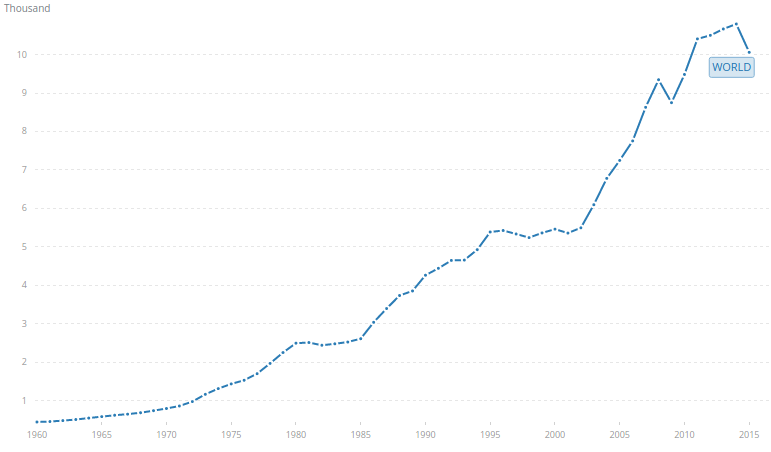
\includegraphics[height=6cm]{../pics/worldbank-GDP-per-capita-1960-2015}
	\caption{World GDP per capita, Credit: \href{http://data.worldbank.org/indicator/NY.GDP.PCAP.CD?end=2015&start=1960}{World Bank, 2017}}
	\end{figure}
}

\begin{frame}[c]{Sources of Innovation}
	\centering
	\Huge{Where does Innovation come from?}
\end{frame}

\frame{
	\frametitle{Sources of Innovation}
	\framesubtitle{Inventors' Main Traits \parencite{rootbernstein89}}
	\begin{itemize}
		\item Have mastered basic tools \& operations in their field/business
		\pause
		\item Understand several fields with diverse perspectives
		\pause
		\item Curious \& more interested in problems than solutions
		\pause
		\item Question status quo
		\pause
		\item Have a sense that all knowledge is unified (system thinking)
	\end{itemize}
}

\frame{
	\frametitle{Theory of Innovation}
	\framesubtitle{Thinking outside the box}
	\begin{block}{Sir MacFarlane Burnet, Nobel Prize:}
		``I think there are dangers for a research man being too well trained in the field he is going to study''
	\end{block}
}

\frame{
	\frametitle{Theory of Innovation}
	\framesubtitle{Other Sources of Innovation}
	\begin{itemize}
		\item Innovation by users (e.g. Loctite case, startup entrepreneurs)
		\pause
		\item Internal R\&D
		\pause
		\item Universities \& Colleges
		\pause
		\item Government-funded R\&D (e.g. Internet)
		\pause
		\item Collaboration with industry peers (e.g. R3 CEV leads a consortium of 75 of the world leading financial institutions)
		\pause
		\item Open Source projects (e.g. Hyperledger, Linux, Tensor Flow, Eclipse, Odoo)
		\pause
		\item Tech Clusters
		\pause
		\item Other?
	\end{itemize}
}

% ------------------ Types and Cycles of Innovation --------------------
\subsection{Types \& Cycles of Innovation}
\frame{
	\frametitle{Theory of Innovation}
	\framesubtitle{Types of Innovation}
	\begin{itemize}
		\item Product Innovation vs. Process Innovation
		\pause
		\item Disruptive Innovation vs. Incremental Innovation
		\pause
		\item Competence-Enhancing Innovation vs. Competence-Destroying Innovation
		\pause
		\item Architectural Innovation vs. Component Innovation
		\pause
		\item Other?
	\end{itemize}
}

\frame{
	\frametitle{Theory of Innovation}
	\framesubtitle{Technological Improvement (Credit: Wgsimon [\href{http://creativecommons.org/licenses/by-sa/3.0}{CC BY-SA 3.0}], via Wikimedia Commons)}
	\begin{figure}
	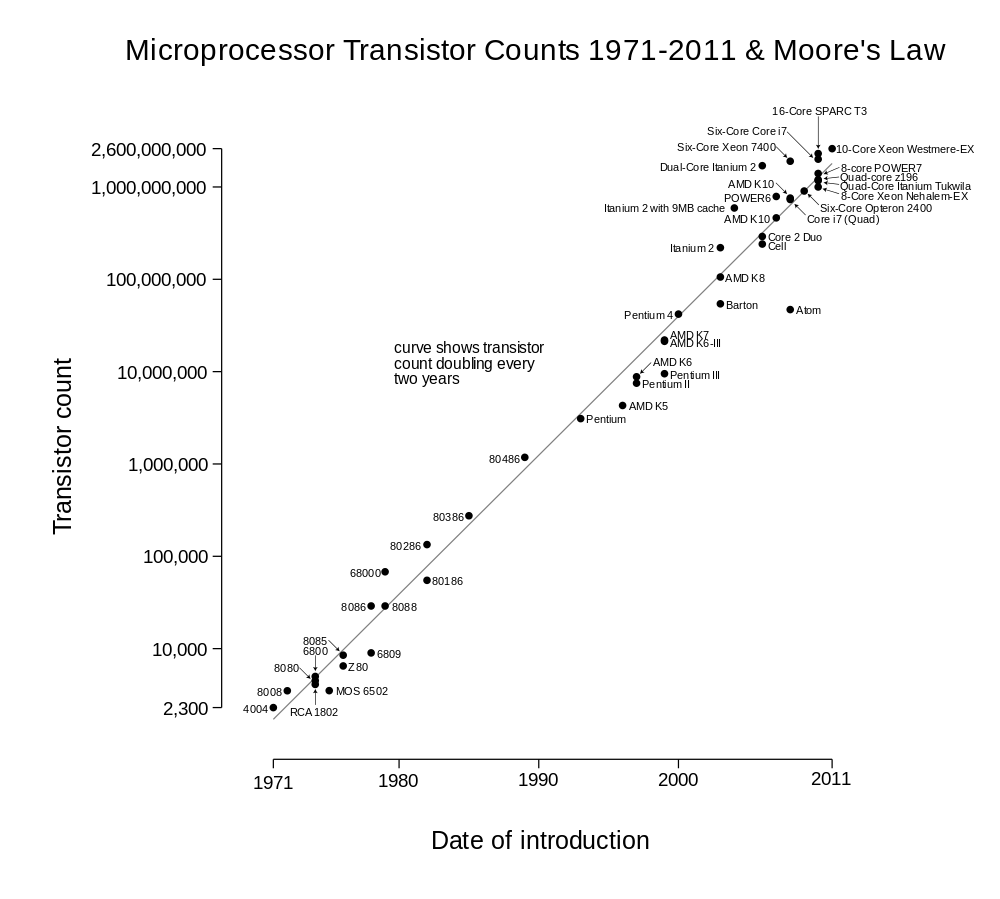
\includegraphics[height=7.5cm]{../pics/Transistor_Count_and_Moores_Law_-_2011}
%	\caption{Transistor Count and Moore's Law -- Credit: Wgsimon [\href{http://creativecommons.org/licenses/by-sa/3.0}{CC BY-SA 3.0}], via Wikimedia Commons}
	\end{figure}
}

\frame{
	\frametitle{Theory of Innovation}
	\framesubtitle{Technological Improvement}
	\begin{alertblock}{Pace of Change}
		How fast does technology improve according to Moore's Law?
	\end{alertblock}
}

\frame{
	\frametitle{Theory of Innovation}
	\framesubtitle{Technological Improvement grows Exponentially (\href{https://mi021.wordpress.com/2013/03/24/is-moore-is-better-the-impact-of-moores-law/}{Heiman, 2013})}
	\begin{figure}
	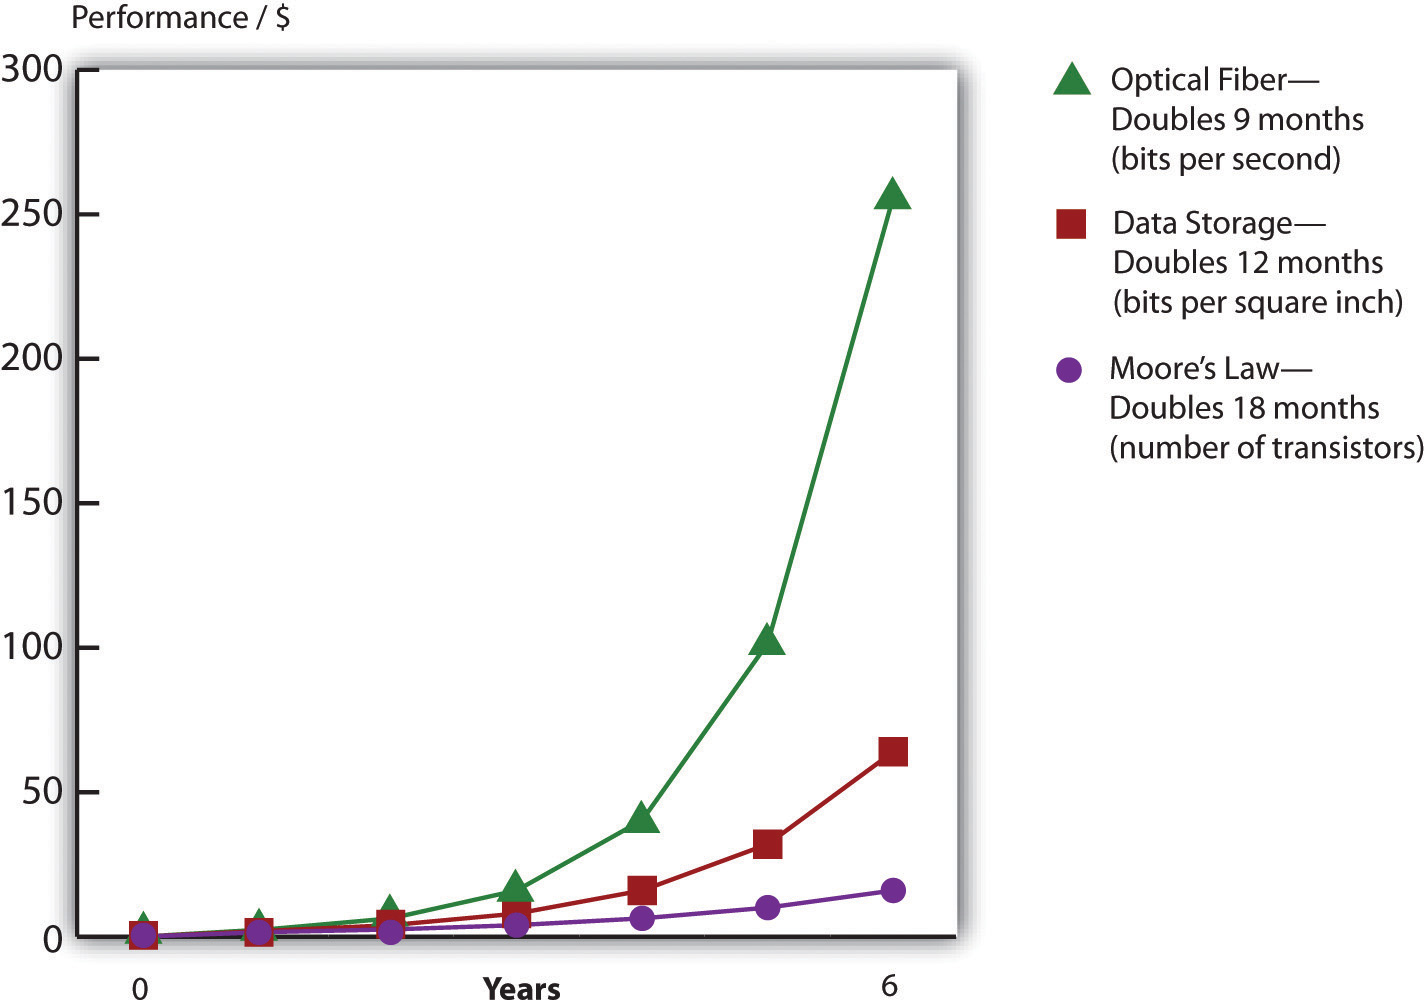
\includegraphics[height=7.5cm]{../pics/advancing-rates-of-technology}
	\end{figure}
}

\frame{
	\frametitle{Theory of Innovation}
	\framesubtitle{Technological Improvement follows and S-Curve (\href{https://www.indybay.org/newsitems/2006/05/18/18240941.php}{Tom Ryun, 2006})}
	\begin{figure}
	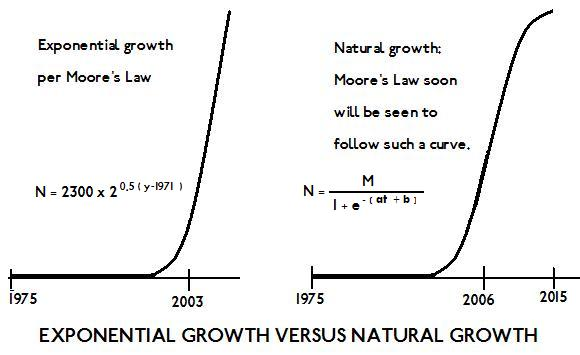
\includegraphics[height=5cm]{../pics/end_of_moores_law_growth_curves}
	\end{figure}
}

\frame{
	\frametitle{Theory of Innovation}
	\framesubtitle{Technological Improvement \& Discontinuous Innovations (\href{http://innovajourney.blogspot.ca/2012/05/s-curve.html}{Gill, 2012})}
	\begin{figure}
	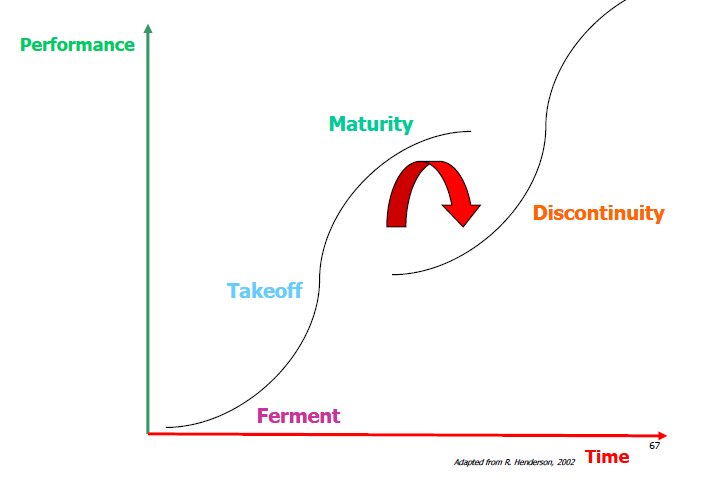
\includegraphics[height=5cm]{../pics/S-Curve-discontinuous}
	\end{figure}
}

\begin{frame}[c]{Diffusion of Innovations}
	\centering
	\Huge{How do innovations spread out and get adopted?}
\end{frame}

\frame{
	\frametitle{Theory of Innovation}
	\framesubtitle{Diffusion of Innovations (\href{http://www.uversity.com/blog/whats-here-vs-whats-next-in-admissions-marketing/}{Leyden})}
	\begin{figure}
	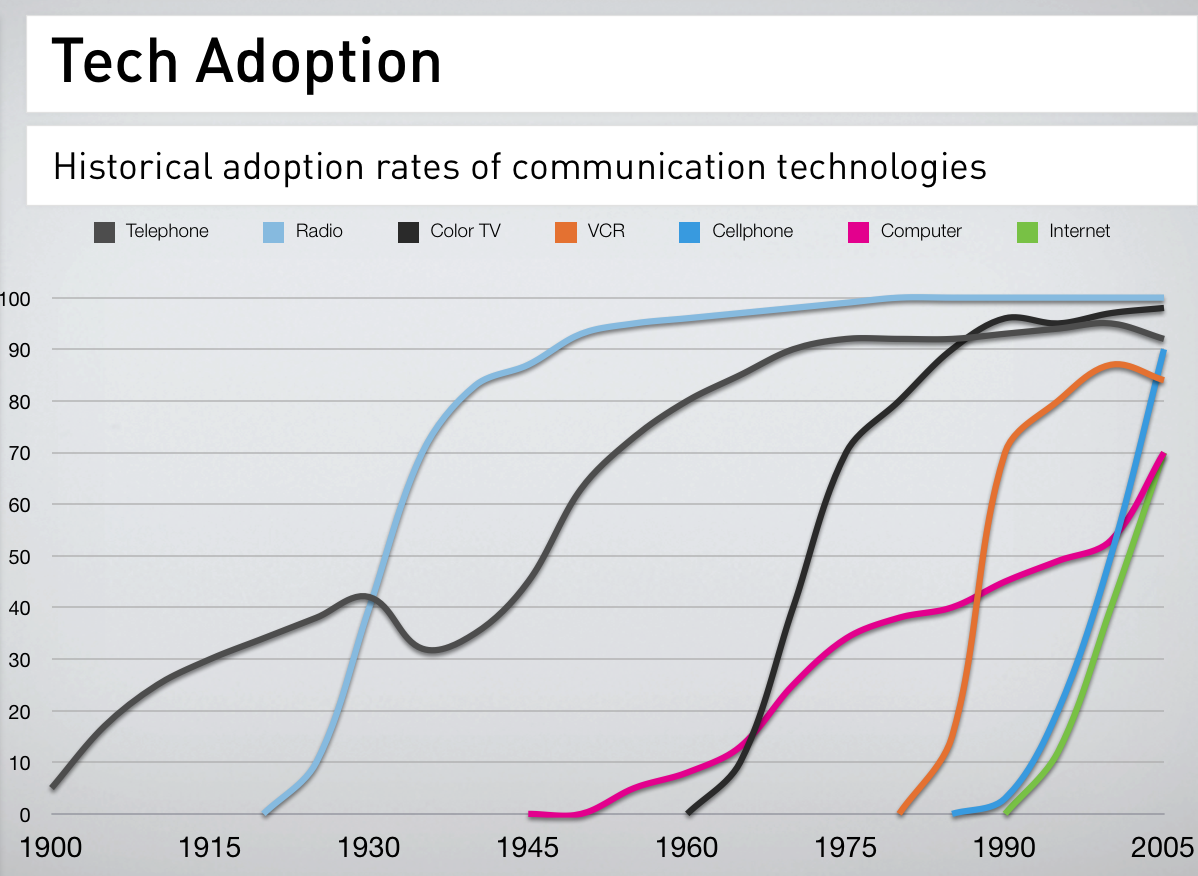
\includegraphics[height=7.5cm]{../pics/Communication-Technology-Adoption-Peter-Leyden}
	\end{figure}
}

\frame{
	\frametitle{Theory of Innovation}
	\framesubtitle{Diffusion of Innovations (\cite{rogers2003diffusion})}
	\begin{figure}
	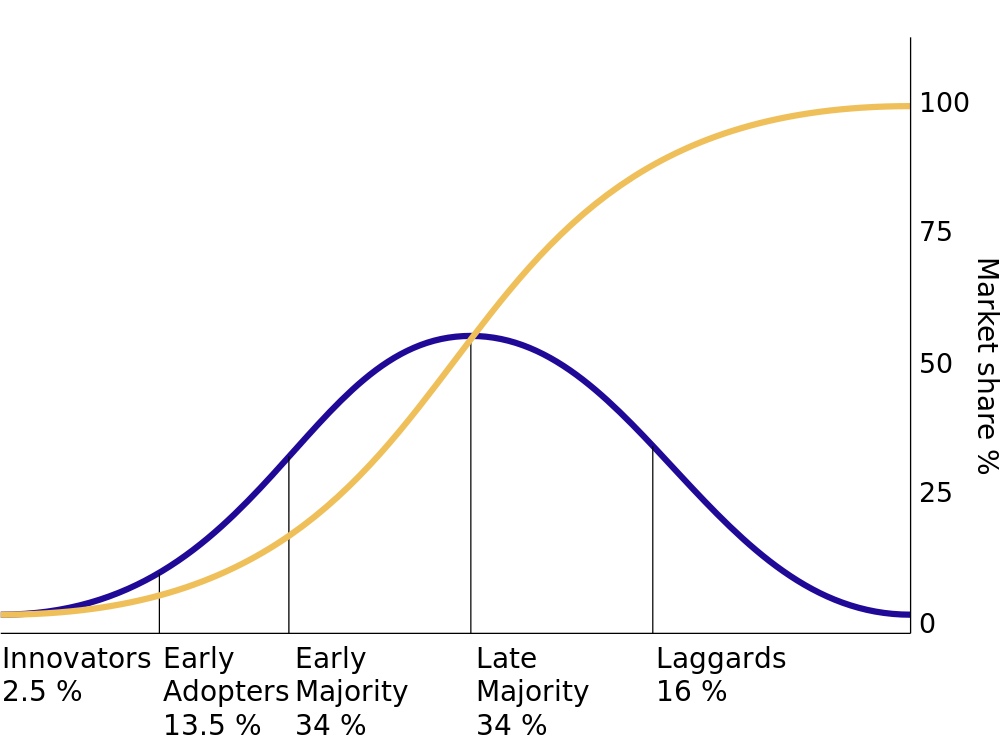
\includegraphics[height=7.5cm]{../pics/Diffusion_of_innovations}
	\end{figure}
}

\frame{
	\frametitle{Theory of Innovation}
	\framesubtitle{Uses \& Limitations of S-Curves}
	\begin{itemize}
		\item Commercialization of Innovations (e.g. improved products, start ups disrupting a market)
		\pause
		\item Forecasting for strategic ventures
		\pause
		\item Other?
	\end{itemize}
}

\begin{frame}[c]{Disruptive Innovations}
	\centering
	\Huge{When to market a disruptive innovation? How good an innovation needs to be to gain adoption?}
\end{frame}

\frame{
	\frametitle{Theory of Innovation}
	\framesubtitle{Disruptive Innovations (\cite{christensen1997innovator})}
	\begin{figure}
	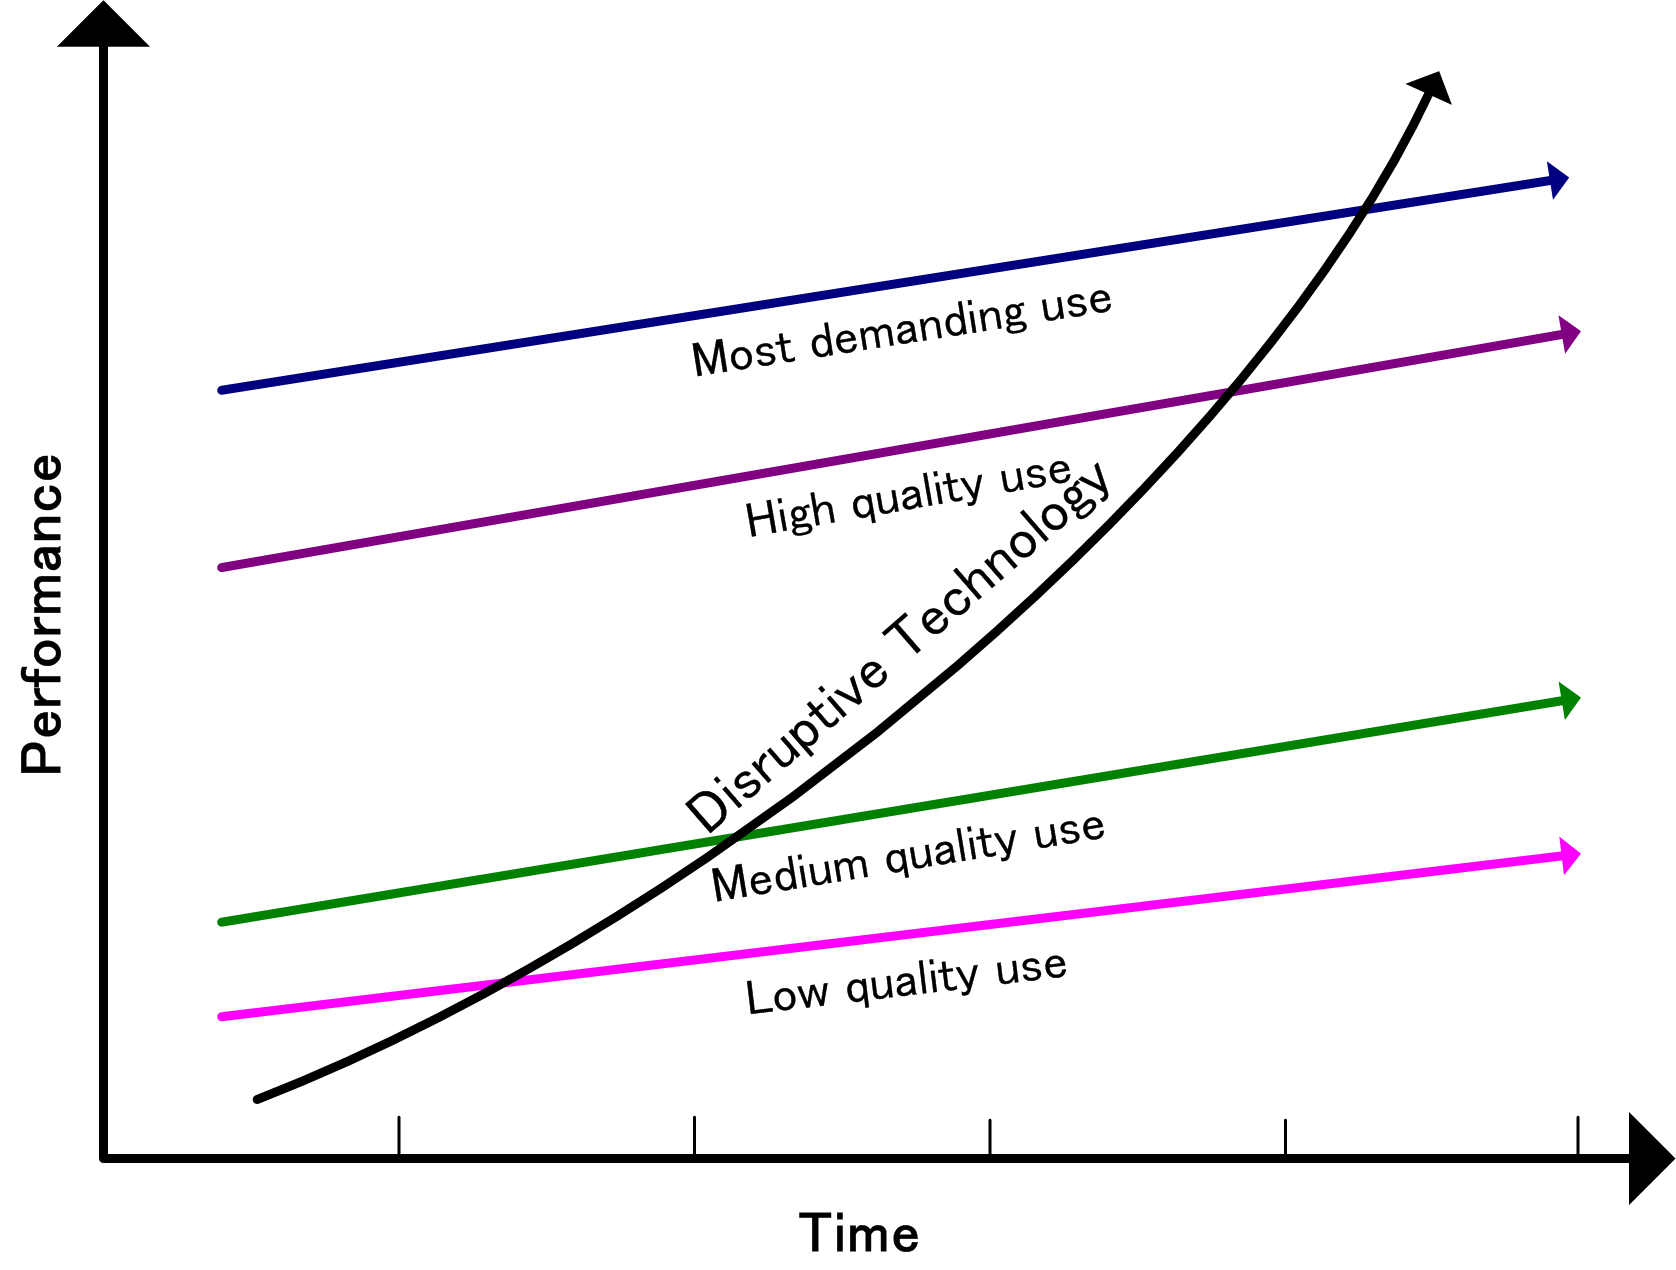
\includegraphics[height=7.5cm]{../pics/Disruptivetechnology}
	\end{figure}
}

\frame{
	\frametitle{Theory of Innovation}
	\framesubtitle{The Innovator's Dilemma (\cite{christensen1997innovator})}
	\begin{alertblock}{The Innovator's Dilemma}
		Should a firm disrupt itself?
	\end{alertblock}
}

\frame{
	\frametitle{Theory of Innovation}
	\framesubtitle{Creative Destruction (\cite{schumpeter2008capitalism})}
	\begin{itemize}
		\item Joseph Schumpeter, born in Austria (1883-1950), then Harvard Professor (1932)
		\pause 
		\item Theory of Economic Innovation (firms die and better ones are created)
		\pause 
		\item Derived from Karl Marx (re. accumulation and annihilation of wealth)
		\pause 
		\item Example: disappearance of Nortel spreads out top engineers in new local firms
	\end{itemize}
}

% ----------------------- Standard Adoption ----------------------------
\subsection{From Innovation to Standards}
\frame{
	\frametitle{Theory of Innovation}
	\framesubtitle{Technology Cycles (Anderson \& Thushman, building on Utterback \& Abernathy)} % TODO cite see Schilling p. 57
	\begin{itemize}
		\item Era of Ferment
		\pause 
			\begin{itemize}
				\item Design Competition
				\item Substitution
			\end{itemize}
		\pause 
		\item Selection of a Dominant Design
		\pause 
		\item Era of Incremental Change
		\pause 
		\item Disruptive Innovation
	\end{itemize}
}

\frame{
	\frametitle{Theory of Innovation}
	\framesubtitle{The Drivers behind the convergence towards a Dominant Design}
	\begin{itemize}
		\item Learning Effects
		\pause 
			\begin{itemize}
				\item Learning Curve: after a while costs of production drop
		\pause 
				\item Technology Spillover
		\pause 
				\item Appearance of mature production tools
		\pause 
				\item Competitors may be better off adopting the same standard
			\end{itemize}
		\pause 
		\item Network Externalities
		\pause 
			\begin{itemize}
				\item Installed Base (e.g. telephone)
		\pause 
				\item Availability of Complementary Goods (e.g. video games for consoles)
			\end{itemize}
		\pause 
		\item Government Regulation (e.g. 4G)
	\end{itemize}
}

\frame{
	\frametitle{Theory of Innovation}
	\framesubtitle{Winner-Take-All Markets}
	\begin{itemize}
		\item Pros
		\pause 
			\begin{itemize}
				\item Learning Effects will lower costs for consumers
				\item Network Externalities will increase value/utility
			\end{itemize}
		\pause 
		\item Cons
		\pause 
			\begin{itemize}
				\item Providers can be in a monopoly position (high prices)
				\item Can slow further innovations
				\item Can kill some businesses (established ones depending on the design, new ones like start ups)
			\end{itemize}
	\end{itemize}
}

\frame{
	\frametitle{Theory of Innovation}
	\framesubtitle{Assessing an Innovation's Value (\cite{kimmauborgne2000})}
	\begin{itemize}
		\item The ``Buyer Utility Map'' is a scorecard to assess value/utility
		\item 6 stages of the buyer experience cycle:
			\begin{enumerate}
				\item Purchase
				\item Delivery
				\item Use
				\item Supplements
				\item Maintenance
				\item Disposal
			\end{enumerate}
		\item 6 utility levers:
			\begin{enumerate}
				\item Customer Productivity
				\item Simplicity
				\item Convenience
				\item Risk
				\item Fun \& Image
				\item Environmental Friendliness
			\end{enumerate}
	\end{itemize}
}

\frame{
	\frametitle{Theory of Innovation}
	\framesubtitle{Assessing an Innovation's Value (\cite{kimmauborgne2000})}
	\begin{figure}
	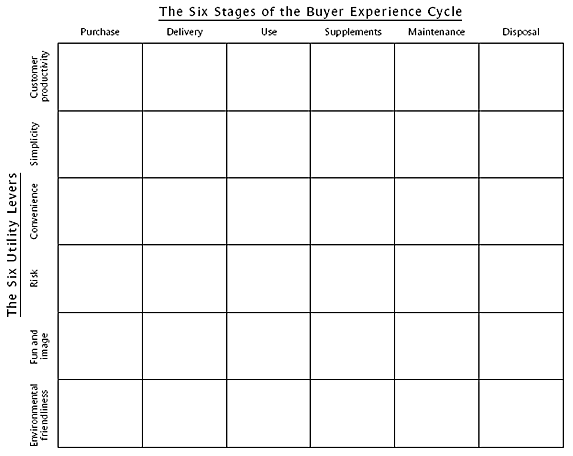
\includegraphics[height=7.5cm]{../pics/buyer-utility-map}
	\end{figure}
}

\frame{
	\frametitle{The 4$^{th}$ Industrial Revolution}
	\framesubtitle{Exercise}
	\begin{alertblock}{Group Work}
		Pick an innovative technology-based product or service and estimate its value for customers.
	\end{alertblock}
}

\frame{
	\frametitle{Theory of Innovation}
	\framesubtitle{References (see more in \cite{schilling2016})}
	%\fullcitebib{schilling2016}
	%\fullcitebib{rootbernstein89}
	% keyword refers to bib file: references-KEYWORD.bib, and to the Tex file: section-KEYWORD.tex
	\printbibliography[keyword=theory-of-innovation]
}

